% !TeX document-id = {117ac6b5-8dd4-4613-9231-0768b5815107}
%pdflatex -shell-escape exos.tex
%pythontex exos.tex
%pdflatex -shell-escape exos.tex
% !TeX TXS-program:compile = txs:///pdflatex/[--shell-escape]
%http://marin.jb.free.fr/latex/
\documentclass[12pt,french]{report}
\usepackage[utf8]{inputenc}
\usepackage{array,multicol,multirow,enumerate,eurosym,latexsym,fourier,bbding,pifont}
\usepackage{graphicx}         % images
\usepackage{verbatim} 
\usepackage{fourier}
\usepackage{graphicx,pst-all}
\usepackage{tabularx}
\usepackage [alwaysadjust]{paralist}
\usepackage{amsmath,amsfonts,amsthm,amssymb,geometry}
\usepackage{fancyhdr}
\usepackage{mathrsfs}  
\usepackage{pstricks,pst-plot,pst-text,pst-tree,pstricks-add,pst-eps,pst-fill,pst-node,pst-math}
\usepackage{euscript,amsfonts,eepic,color}
\usepackage{ifthen,fp}
\newcommand{\Calig}[1]{\ensuremath{\mathscr{#1}}}              
\usepackage{babel}
\usepackage{xcolor}
\usepackage{minted}
\usepackage{pythontex}
\usepackage{multicol}
\usepackage[most]{tcolorbox}
\usepackage{fancyhdr}
\setlength{\parindent}{0pt}
\usepackage{ulem}
\includeonly{exos}
\usepackage{pdfpages}
\usepackage[np]{numprint}
\geometry{vmargin=15mm,hmargin=5mm}
\pagestyle{empty}
\setlength\columnsep{5mm}
\renewcommand{\thesection}{\Roman{section}}
\renewcommand{\thesubsection}{\arabic{subsection}}
\renewcommand{\thesubsubsection}{\arabic{subsubsection}}
\newcounter{npb}
\setcounter{npb}{0}
\newcommand{\exo}{
    \stepcounter{npb}
    {\textbf{$\triangleright$ \underline{Exercice \arabic{npb} }}}
}
\newcounter{sf}
\setcounter{sf}{0}
\newcommand{\s}{
    \stepcounter{sf}
    {\textbf{ \fbox{SF \arabic{sf} }}}
}
\usepackage{lscape}
\usepackage{tikz}
\usepackage{metalogo}
\usepackage{hyperref}
\title{\huge{\fbox{Projet de validation du bloc 2} } \\\vskip1 cm Proposition de cours\\\vskip1 cm \huge{\fbox{Thème choisi : les algorithmes gloutons }}}      % renseigne le titre
\author{Aude Duhem et Patrice Nicolas}           %   "   "   l'auteur
\date{juillet 2019}
\pagestyle{headings} 
\begin{document}
	\maketitle
\tableofcontents
  \lhead {DIU }
    \chead{Enseigner l'informatique au lycée}
    \rhead{Bloc 2}
      \renewcommand{\headrulewidth}{0.5pt}
      \lfoot{                      }\cfoot{Page \thepage}\rfoot{\textsf{Aude Duhem et  Patrice Nicolas}}
    \pagestyle{fancy}
    \renewcommand{\footrulewidth}{0.4pt}
    \normalsize
\chapter{Support pédagogique}
\section{Prérequis}
\begin{itemize}[$\bullet$]
\item Types de base, listes, dictionnaires;
\item  instruction IF, boucles FOR et WHILE ; 
\item spécification, définition et appel de fonctions ;
\item  importation de modules tels que random et time.
\item connaissance des notions de complexité, terminaison et correction des algorithmes
\item algorithmes de tri (dont complexité ) (car les algorithmes gloutons supposent d'avoir des valeurs triées)
\end{itemize}
\section{Notions abordées dans le cadre du programme NSI Première}
\begin{tabular}{|p{4cm}|p{6cm}|p{8cm}|}
\hline
Contenus&Capacités attendues&Commentaires\\
\hline
\multicolumn{3}{|c|}{Algorithmique}\\
\hline
Algorithmes gloutons&Résoudre un problème grâce à un algorithme glouton& Exemples : problèmes du sac à dos ou du rendu de monnaie.\\
&& Les algorithmes gloutons constituent une méthode algorithmique parmi d'autres qui seront vues en terminale.\\
\hline
	
\end{tabular}
\section{Situation dans l’année scolaire}
Cette séquence vient en milieu d’année, au minimum après les prérequis .\\
  Durée : 8 heures de 55 min.
  \section{Compétences attendues en fin de séance}
  \begin{itemize}[$\bullet$]
  \item connaissance du principe des algorithmes gloutons et de ses faiblesses
  \item sensibilisation à la notion d'optimisation
  \item connaissance des deux algorithmes de référence au programme : 
   \item Approfondissement des types tableaux de données et dictionnaires
 \item Approfondissement des notions de complexité, terminaison, correction d'un algorithme
\end{itemize} 
\section{Modalité d'évaluation}
\begin{itemize}[$\bullet$]
	\item Évaluation des corrections orales des élèves en séances 
	\item Interrogation sommative en séance 6 
	\item Évaluation des compte-rendu des TP1 et TP2
\end{itemize} 
\chapter{Progression envisagée}
\section{séance 1 - 1 h - séance débranchée}
\subsection{Activités d'introduction du principe des algorithmes gloutons (15-20 min) - cf. annexe A}
introduction faite à partir de deux activités : un exemple pour introduire optimisation/méthode gloutonne et un problème du rendu de monnaie.\\
Travail proposé en groupe pour amener les élèves à découvrir les notions de problèmes d'optimisation, d' algorithme glouton et la "solution" du problème de rendu de monnaie.
\subsection{synthèse sur le cahier de cours (20 min)-  - cf. annexe B}
Cours jusqu'au III A (inclus)
Définition concept de problème d'optimisation et d'algorithme glouton\\
Principe de l'algorithme du rendu de monnaie\\
énoncé en pseudo-code +\\
\subsection{Exercice d'application (15 min) - cf. annexe C}
exercice 1  - exercice où l'algorithme glouton trouve la solution optimale
\paragraph{Devoirs pour la séance suivante : finir l' exercice }
\section{séance 2 - 2 h - TP}
\subsection{Retour sur la séance précédente (10 min)}
Réactivation des connaissances acquises lors de la séance précédente.\\
Projection et explications à l’oral de l’exercice 1 (annexe C) par un élève
\subsection{Première partie de la séance (1 h 30 min)}
TP de rendu de monnaie à programmer en Python\\
Difficultés croissantes\\
Exercice 4 (de la feuille d'exercices) à proposer pour les élèves rapides
\subsection{Deuxième partie de la séance (0 h 20 min)}
Exercices 2 et 3 - Exercices de rendu de monnaie où l'algorithme glouton ne trouve pas la solution optimale
\paragraph{Devoirs pour la séance suivante :\\
- finir le compte-rendu de TP\\
- finir les exercices 2 et 3}
\section{séance 3 - 1h - séance débranchée}
\subsection{Retour sur la séance précédente (10 min)}
Réactivation des connaissances acquises lors de la séance précédente.\\
Projection et explications à l’oral des exercices 2 et 3 (annexe C) par un élève
\subsection{synthèse sur le cahier de cours (35 min)-  - cf. annexe B}
Paragraphes III B et III C :Complexité, terminaison et correction de l'algorithme du rendu de monnaie\\

\subsection{Découverte du principe de l'algorithme du sac à dos (10 min)}
Travail de groupe : exercice 5 - exercice d'introduction de l'algorithme du sac a dos

\paragraph{Devoirs pour la séance suivante : finir l'activité }
\section{séance 4 - 1h - séance débranchée}
\subsection{Retour sur la séance précédente (5 min)}
Réactivation des connaissances acquises lors de la séance précédente.\\
Projection et explications à l’oral de l'activité par chaque groupe
\subsection{synthèse sur le cahier de cours (30 min)-  - cf. annexe B}
Algorithme du sac à dos - Paragraphe IV
définition de façon "littérale", sensibilisation au formalisme si le groupe s'y prête et si le groupe a vu les notations en cours de mathématiques.\\
critères\\
énoncé en pseudo-code+ complexité et terminaison\\
\subsection{Exercice d'application (15 min) - cf. annexe C}
exercice 6 - exercice à la main pour vérifier que l'algorithme du sac à dos est compris\\
Exercice 7  - exercice moins guidé de l'algorithme du sac et permettant de découvrir des méthodes à employer en Python pour effectuer des tris selon des critères.
\paragraph{Devoirs pour la séance suivante :
	Retravailler le cours sur le sac à dos et finir l'exercice 7}

\section{séance 5 - 2 h - TP }
\subsection{Retour sur la séance précédente (10 min)}
Projection et explications à l’oral de l'exercice 7 (annexe C) par un élève
\subsection{Travail de groupe - 15 min }
Élaboration d'une fiche mémorisation/résumé de cours, en groupe (forme libre : carte mentale, résumé linéaire, ...)\\
Le professeur circule pour vérifier que les compétences attendues sont bien cernées.\\
Les productions ainsi produites sont mises à disposition du groupe classe sur l'ENT via un espace partagé.\\

\subsection{Fin de la séance (1 h 30 min)}
TP de sac à dos\\
Exercice 8 (de la feuille d'exercices) à proposer pour les élèves rapides
\paragraph{Devoirs pour la séance suivante : 
	se préparer pour l'évaluation et demander à chacun une petite recherche ciblée (2 élèves par attendu) afin de pouvoir remplir, ensemble, la frise chronologique des algorithmes gloutons\\
}
\section{séance 6 - 1h }
\subsection{Évaluation (30 min) (cf. annexe E)}
\subsection{Correction à l'oral avec les élèves de l'évaluation (10 min) (cf. annexe E)}
\subsection{Point bilan sur les nouveaux termes rencontrés dans cette séance (10 min) (cf. annexe F)}
Au fur et à mesure de l’année un lexique est constitué avec les élèves.
Projection et explications de l’annexe F qui viendra amender ce lexique.
\subsection{Frise chronologique du chapitre à compléter  (10 min) (cf. annexe H)}
En fonction des apports des élèves, esquisser une frise chronologique du chapitre\\
\paragraph{Devoirs pour la séance suivante : rendre le compte-rendu du TP2\\
}
\chapter{Répartition des tâches}
Après avoir respectivement fait des recherches individuellement,
nous avons en commun réfléchi à une progression envisageable et nous sommes donnés un premier axe d'approche :
\begin {itemize}
\item Patrice est le responsable principal de l'algorithme du sac à dos
\item Aude est la responsable principale de l'algorithme du rendu de monnaie
\end{itemize}
Voici la répartition du travail de chacun :\\

\begin{tabular}{|c|m{7cm}|m{7cm}|}
\hline
&Aude Duhem&Patrice Nicolas\\
\hline
Support pédagogique&Recherche et conception du support&\\
\hline
Progression envisagée&Réflexion conjointe&Réflexion conjointe\\
&Finalisation&\\
&saisie et mise en page&\\
\hline
Actvivité d'introduction&Recherche, conception et mise en page de l'activité problème de monnaie &Recherche, conception de l'activité maître nageur\\
\hline
Support de cours&Recherche et conception conjointe&Recherche et conception conjointe\\
\hline
Feuille d'exercices&Recherche et conception des exercices 1 à 4&Recherche et conception des exercices 5 à 8\\
\hline
TP1 rendu de monnaie&recherche, concept, tests, corrigé et compléments pédagogiques&\\
\hline
TP sac à dos&&recherche, concept, tests, corrigé et compléments pédagogiques\\
\hline
Evaluation&Recherche et conception conjointe&Recherche et conception conjointe\\
\hline
Notions mises au lexique&Recherche et conception conjointe&Recherche et conception conjointe\\
\hline

Frise chronologique&Recherche du site ou de l'application adéquate, 
recherches et élaboration de la frise&\\
\hline
\end{tabular}
\appendix

\chapter{Activités d'introduction}
Ce support propose deux activités d'introduction aux principes de problème d'optimisation, d'algorithme glouton et du problème de rendu de monnaie. \\

\section{\textbf{Déroulé envisagé }}
\subsection{\textbf{introduction orale }}
Dans la vie courante, il y  a beaucoup de situations où on cherche la solution la plus optimale face à un problème donné tel que : 
\begin{itemize}[$\bullet$]
	\item Rendre la monnaie avec le moins de pièces : problème du caissier;
	\item  ranger son sac de façon optimisée  : problème du sac à dos;
	\item ranger des objets avec un nombre minimum de boîtes   : bin packing;
	\item trouver le plus court chemin : Algorithme de Djikstra \\
\end{itemize} 
Nous allons pour introduire ce chapitre, nous familiariser à la notion de problème d'optimisation et au premier problème cité.
\subsection{\textbf{Travail de recherche en groupe}}
Le professeur distribue l'énoncé des deux activités à des élèves répartis en groupe de 3\\
Les laisser chercher vingt minutes par groupe de 3/4 élèves et faire une synthèse tous ensemble.\\

\hrule
\bigskip
\textbf{Intérêt} : fixer sur des exemples concrets des principes de problème d'optimisation et d'algorithme glouton et du problème du rendu de monnaie\\
\hrule

\hrule
\begin{center}
	
\end{center} 
\section{Compléments pédagogiques de l'activité 1 :}
Activité permettant de sensibiliser les élèves aux notions de problèmes d'optimisation en abordant deux approches : l'approche naïve et l'approche gloutonne. 
Les élèves n'obtiendront pas la solution optimale car on a volontairement pas donné suffisamment d'informations.
\section{Compléments pédagogiques de l'activité 2 :}
Il est possible, que pour le problème du rendu de monnaie, que deux méthodes "sortent" : l'algorithme glouton naïf et celui où on fait des divisions au lieu des soustractions.\\
Les faire conclure qu'on arrivera de toute façon au même rendu de monnaie.\\
Et les faire trouver par tâtonnement une définition avec leurs mots des principes de problème d'optimisation et d'algorithme glouton.\\
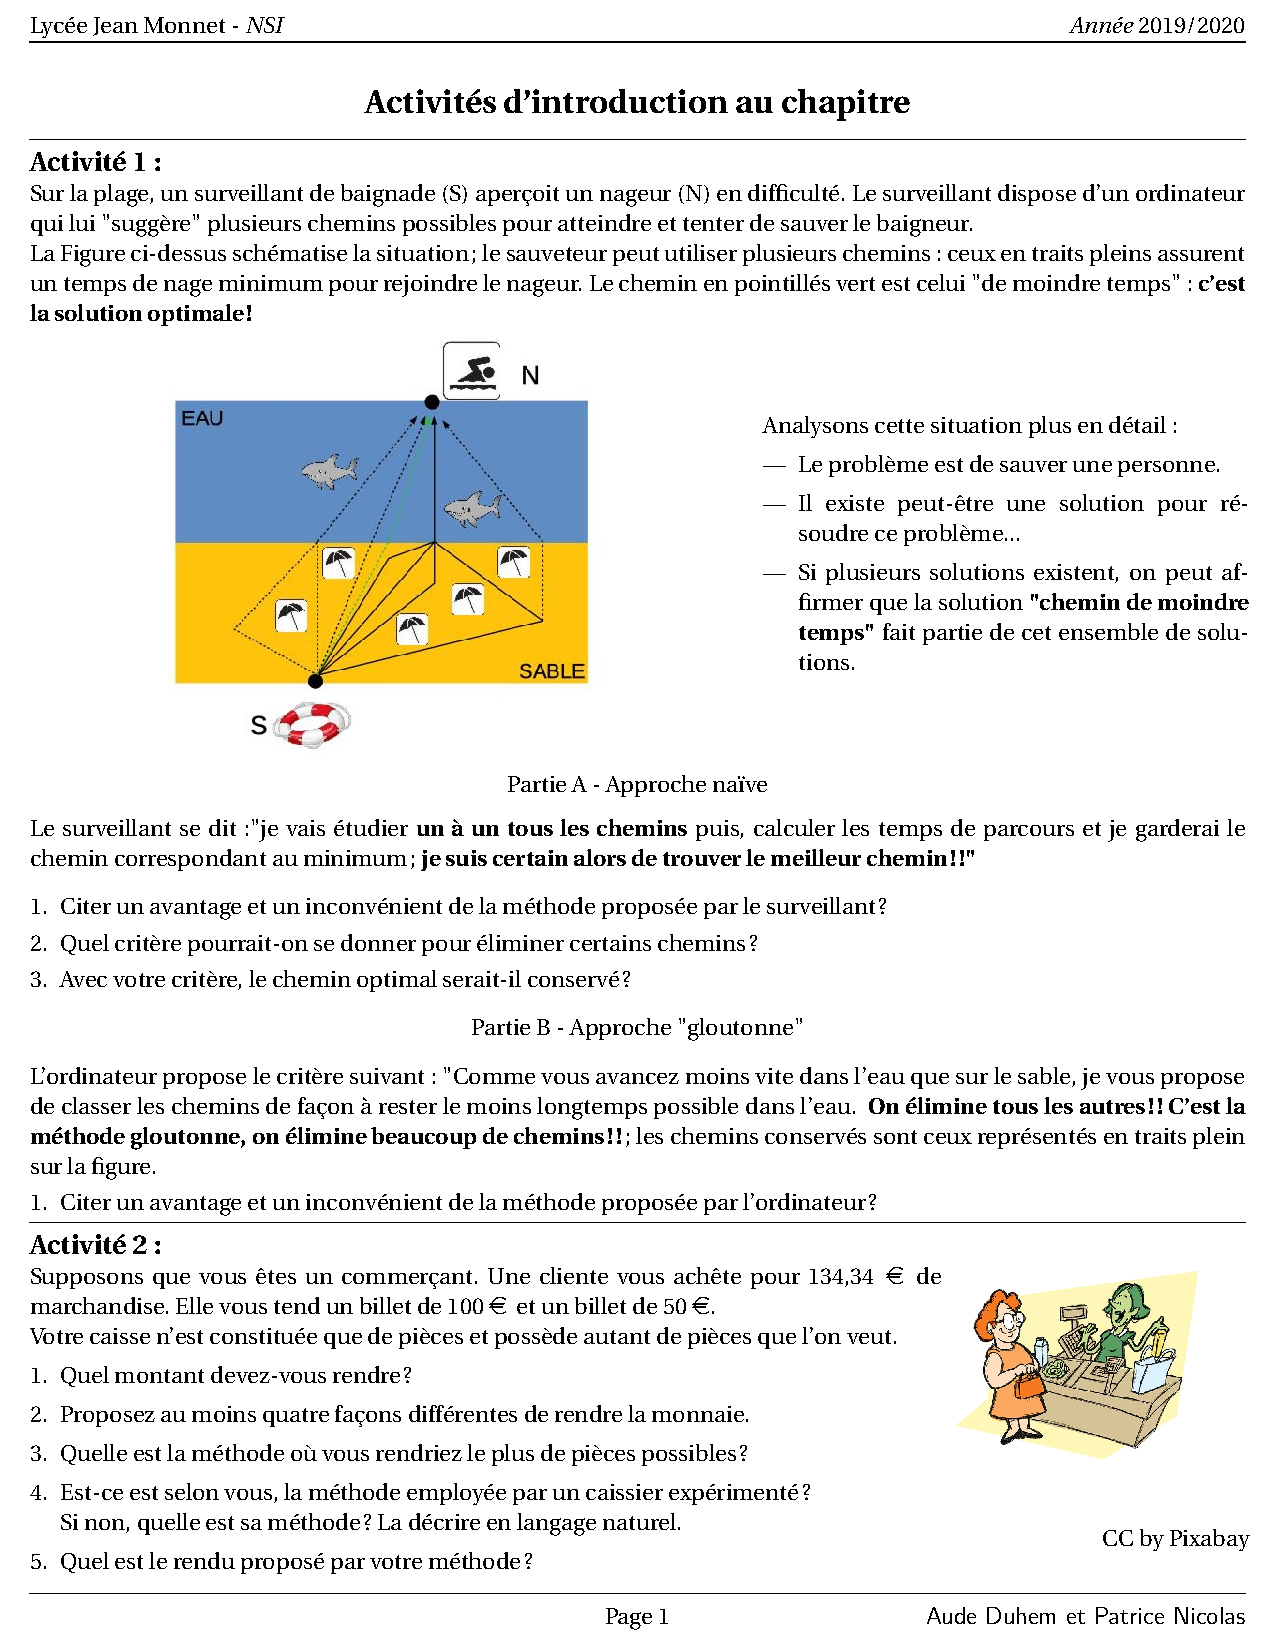
\includepdf[pages=-]{annexe1.pdf}
% ...

\chapter{Support de cours}
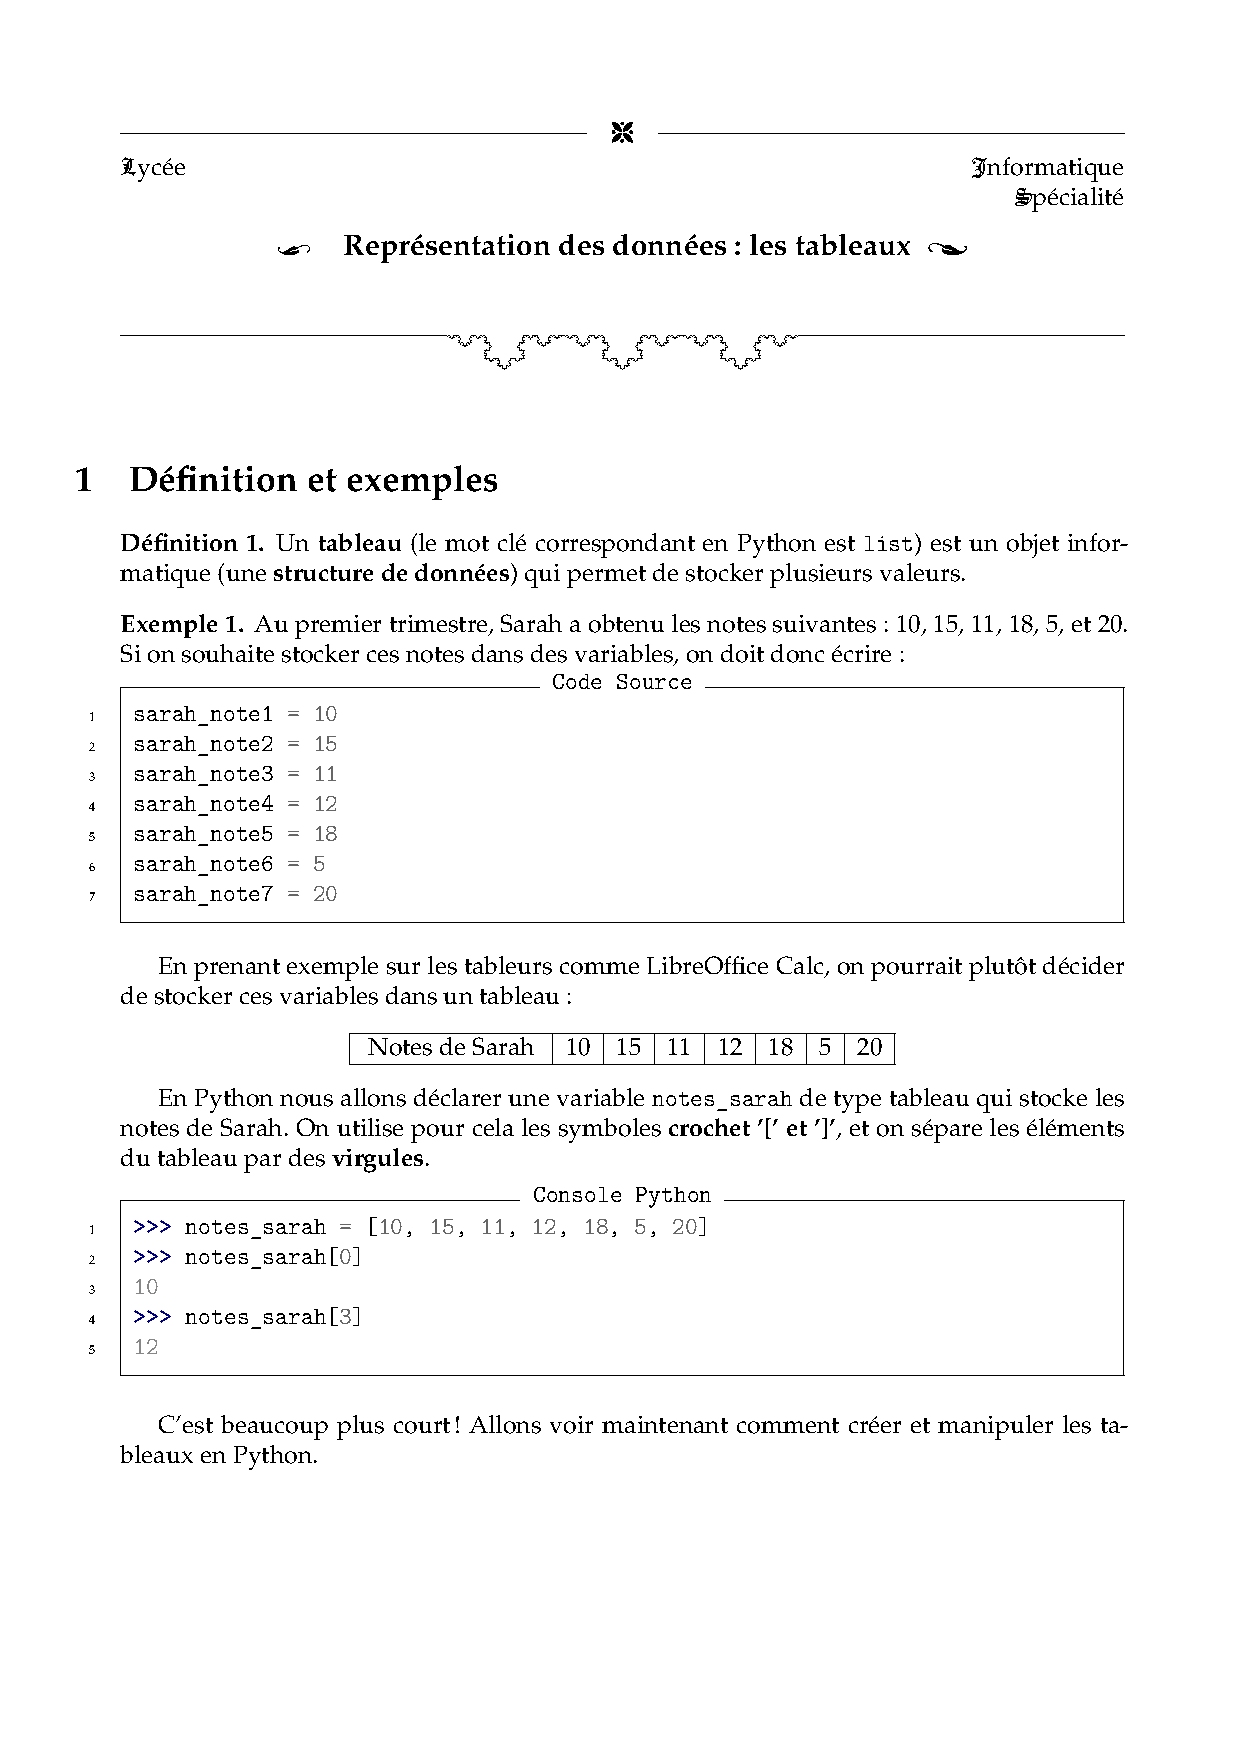
\includepdf[pages=-]{cours.pdf}
%...
\chapter{Feuille d'exercices}
Sur cette feuille d'exercices, sont proposés des exercices portant sur le thème des algorithmes gloutons
\section{Compléments pédagogiques des exercices 1 à 3 :}
\begin{center} Ces trois exercices sont débranchés. \end{center}
Ces trois premiers exercices portent sur le problème du rendu de monnaie.\\
L'exercice 1 permet de tester à la main l'algorithme du rendu de monnaie avec un système canonique et de préparer les élèves au TP1.
Les exercices 2 et 3 sont des exercices où les systèmes de monnaie ne sont pas canoniques. On a veillé dans ces exercices à leur donner un contexte.
\section{Compléments pédagogiques de l'exercice 4}
\begin{center} Cet exercice est branché. \end{center}
Cet exercice est un exercice plus ouvert car il ne fait pas appel aux deux algorithmes gloutons vus en classe et sera donc proposé aux élèves les plus rapides.
\section{Compléments pédagogiques de l'exercice 5}
\begin{center} Cet exercice est débranché. \end{center}
Cet exercice est un exercice d'introduction au problème du sac à dos et permet d'introduire le TP2.
\section{Compléments pédagogiques des exercices 6 à 7 :}
\begin{center} Ces deux exercices sont débranchés. \end{center}
L'exercice 6 permet de tester à la main l'algorithme du sac à dos et de vérifier si le principe est bien compris.
L'exercice 7 est un exercice moins guidé de l'algorithme du sac et qui permet la découverte des méthodes à employer en Python pour effectuer des tris selon des critères.
\section{Compléments pédagogiques de l'exercice 8}
\begin{center} Cet exercice est branché. \end{center}
Cet exercice est un exercice plus ouvert permettant de comparer la méthode brute du sac à dos avec les critères de l'algorithme du sac à dos.
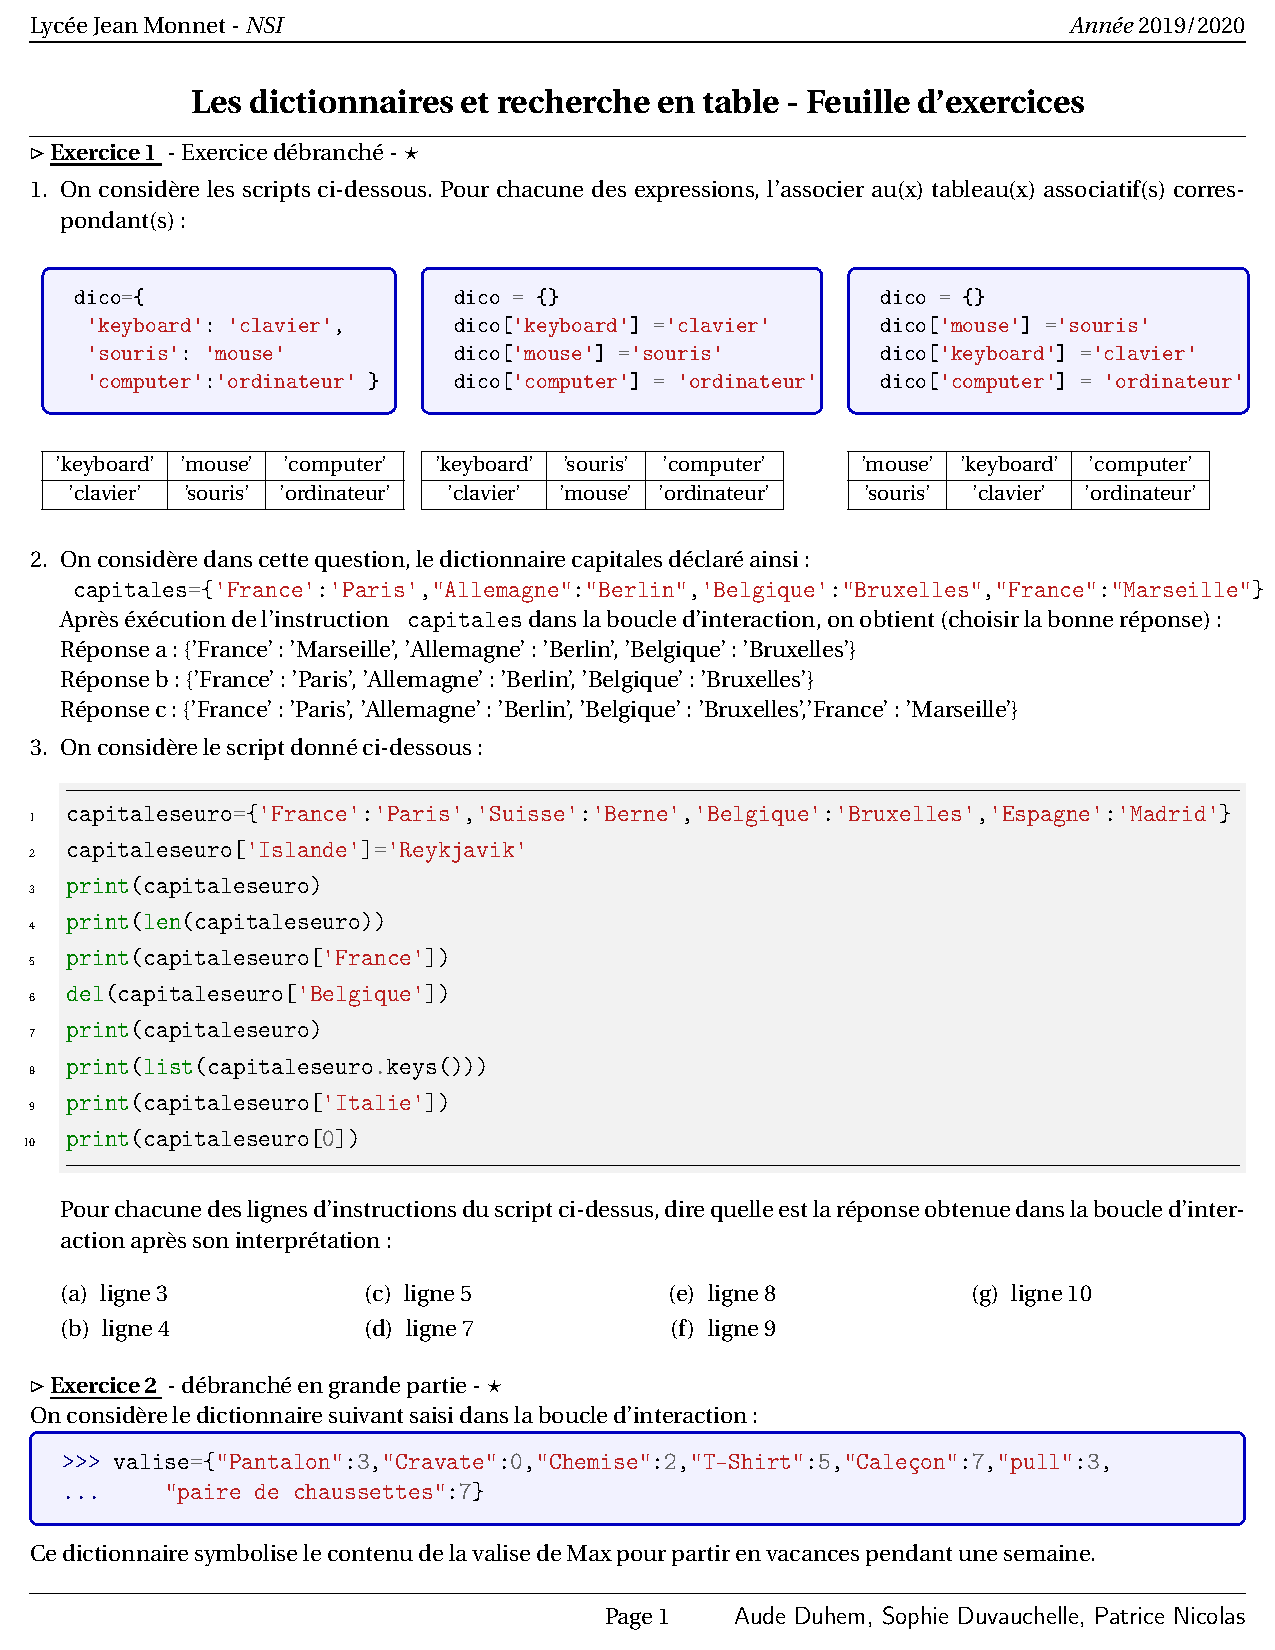
\includepdf[pages=-]{exos.pdf}
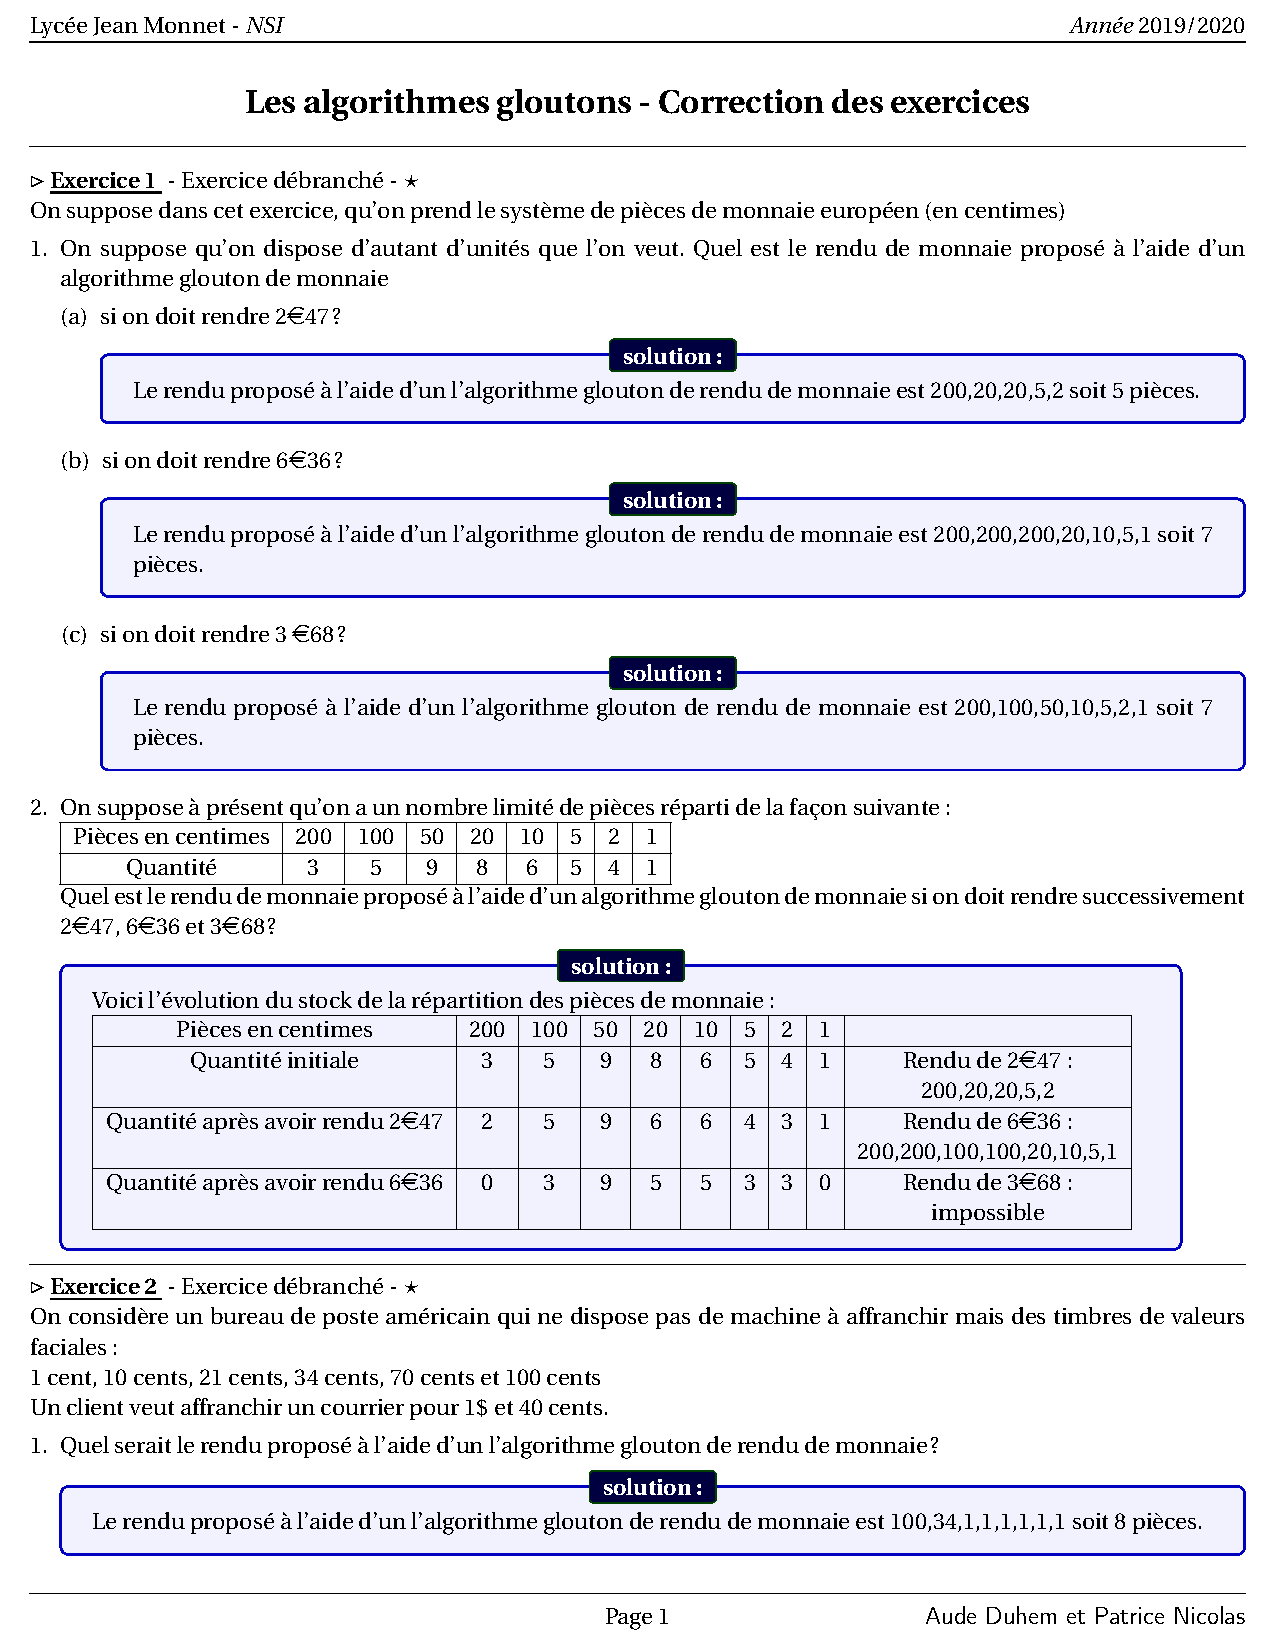
\includepdf[pages=-]{exoscor.pdf}

\chapter{TP}
Deux TP sont prévus :
\begin{itemize}
	\item TP1 : rendu de monnaie
	\item TP2 : sac à dos
\end{itemize}

\section{Compléments pédagogiques du TP1 :}
Le TP1 s'instaure dans la continuité de ce qui a été fait en classe avant.\\
Prérequis : les mêmes que pour toute la séance.\\
Les parties sont en ordre croissant de difficulté et ont été préparées via l'exercice 1 fait en classe.\\
Remarque : le système de monnaie étant généralement de petite taille, les listes seront supposées prétriées 
\medskip
\subsection{Principe général du TP }
But du TP : programmer un appareil qui rend automatiquement la monnaie à l'aide d'un algorithme glouton de rendu de monnaie.\\
Dans les parties I et II : La caisse est sous la forme d'une liste contenant les valeurs des pièces par ordre décroissant. On suppose que l'on dispose d'autant de pièces que l'on veut.\\ 
Partie I : \\
but : écrire une caisse sous forme d'une liste et écrire une fonction qui retourne un rendu de monnaie sous la forme d'une liste \\
Partie II : \\
but : écrire une fonction qui retourne un rendu de monnaie sous la forme d'une liste de liste\\
Partie III : \\
La caisse est à présent sous la forme d'un dictionnaire qui prend en compte le nombre de pièces de chaque catégorie\\
but : écrire une caisse sous forme d'un tel dictionnaire et une fonction qui retourne un rendu de monnaie sous la forme d'un dictionnaire indiquant les quantités prises pour chaque pièce si c'est possible ou un message si le rendu est impossible \\
\subsection{Objectifs }
\begin{itemize}[$\bullet$]
	\item vérifier la compréhension du principe de l'algorithme glouton du rendu de monnaie
	\item Revoir les différentes structures de données (de la liste simple, aux dictionnaires via les listes de listes)
	\item réinvestir les boucles et les tests
	\item Mettre en oeuvre un algorithme glouton en Python
\end{itemize}
\subsection{Difficultés anticipées }
\begin{enumerate}
	\item comprendre la démarche à suivre pour résoudre le problème
	\item Manipuler une liste dans une liste
	\item Manipuler un dictionnaire et confusion clé/valeur dans un dictionnaire
\end{enumerate}
\subsection{Remédiation envisagées }
\begin{enumerate}
	\item ré-explication du principe
	\item donner des exemples de cas simples
	\item prendre des exemples où la clé n'est pas un nombre, où la manipulation est sans équivoque
\end{enumerate}
\section{Compléments pédagogiques du TP2 :}
\subsection{Principe général du TP }
Ce TP arrive en fin de séquence sur les gloutons ; il permet de réinvestir la notion de tri et viser davantage à comparer les réponses des algorithmes gloutons qu'à écrire les algorithmes eux-mêmes.\\
Partie I le tri:\\
On revient sur un principe de tri (supposé connu et maitrisé) ; l'élève propose une modification possible de son Tri Classique afin de l'adapter à un tableau à 2 dimensions.
On rappelle brièvement le caractère immuable des tuples qui rend plus compliqué le tri d'une liste de tuples.
On demande à l'élève de s'emparer de quelques lignes de la documentation officielle
Python (éventuellement en anglais) afin d'analyser une syntaxe nouvelle. La notion de fonction lambda n'est pas introduite en tant que telle.\\
 Partie II : Exécution de l'algorithme du sac à dos selon trois critères.\\
l'élève écrit ses trois algorithmes qui ne différent que par le critère de décision. il teste les codes sur un ensemble de données fourni dans un fichier annexe.
On pourrait demander à un élève très à l'aise, de lire directement dans le fichier.
On compare et commente la réponse des algorithmes : coût en temps, optimalité.
\subsection{Objectifs }
\begin{itemize}[$\bullet$]
	\item réinvestissement des tris
	\item vérifier la compréhension du principe de l'algorithme glouton du sac à dos 
	\item Revoir les différentes structures de données 
	\item réinvestir les boucles et les tests
	\item Mettre en oeuvre un deuxième algorithme glouton en Python
\end{itemize}
\subsection{Difficultés anticipées }
\begin{enumerate}
	\item Remobiliser ses connaissances sur les tris
	\item comprendre la démarche à suivre pour effectuer l' étude des performances des algorithmes

\end{enumerate}
\subsection{Remédiation envisagées }
\begin{enumerate}
	\item ré-explication du principe
	\item donner des exemples 
\end{enumerate}
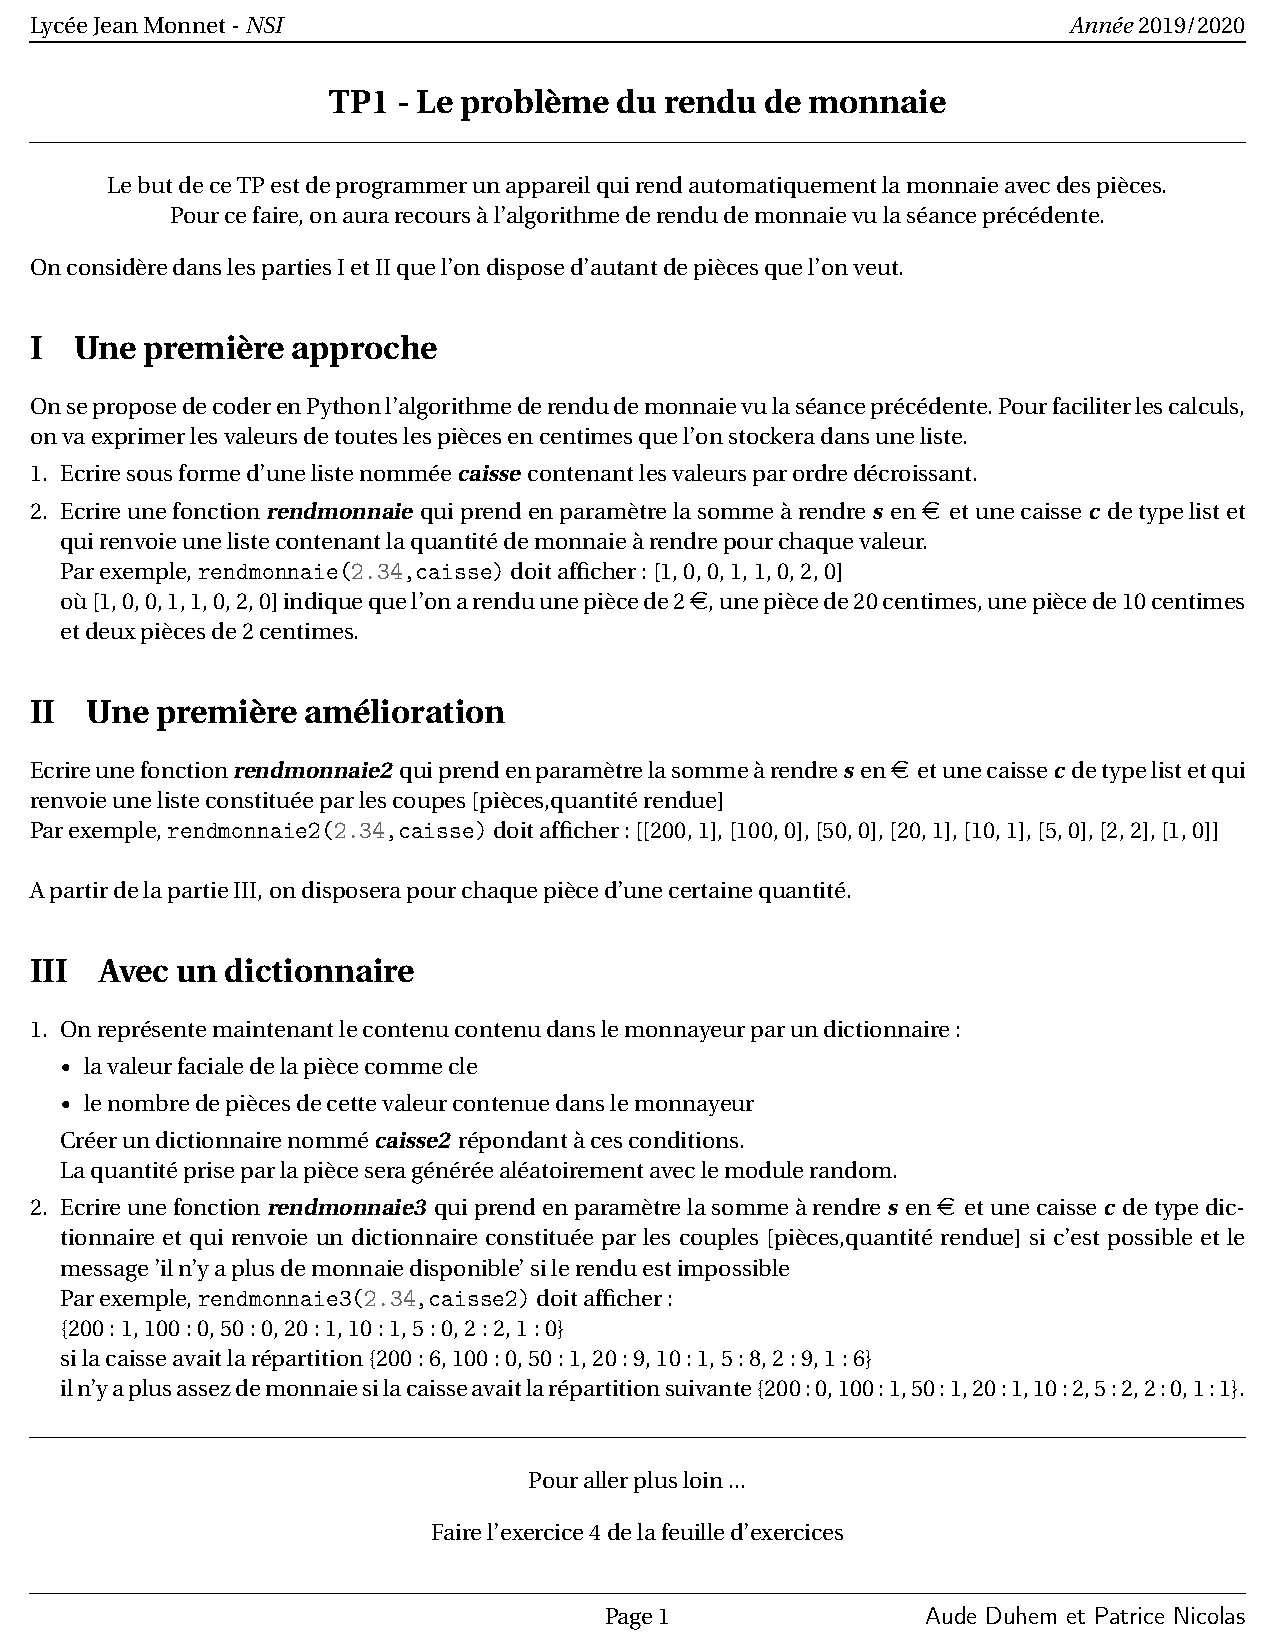
\includepdf[pages=-]{TP1.pdf}
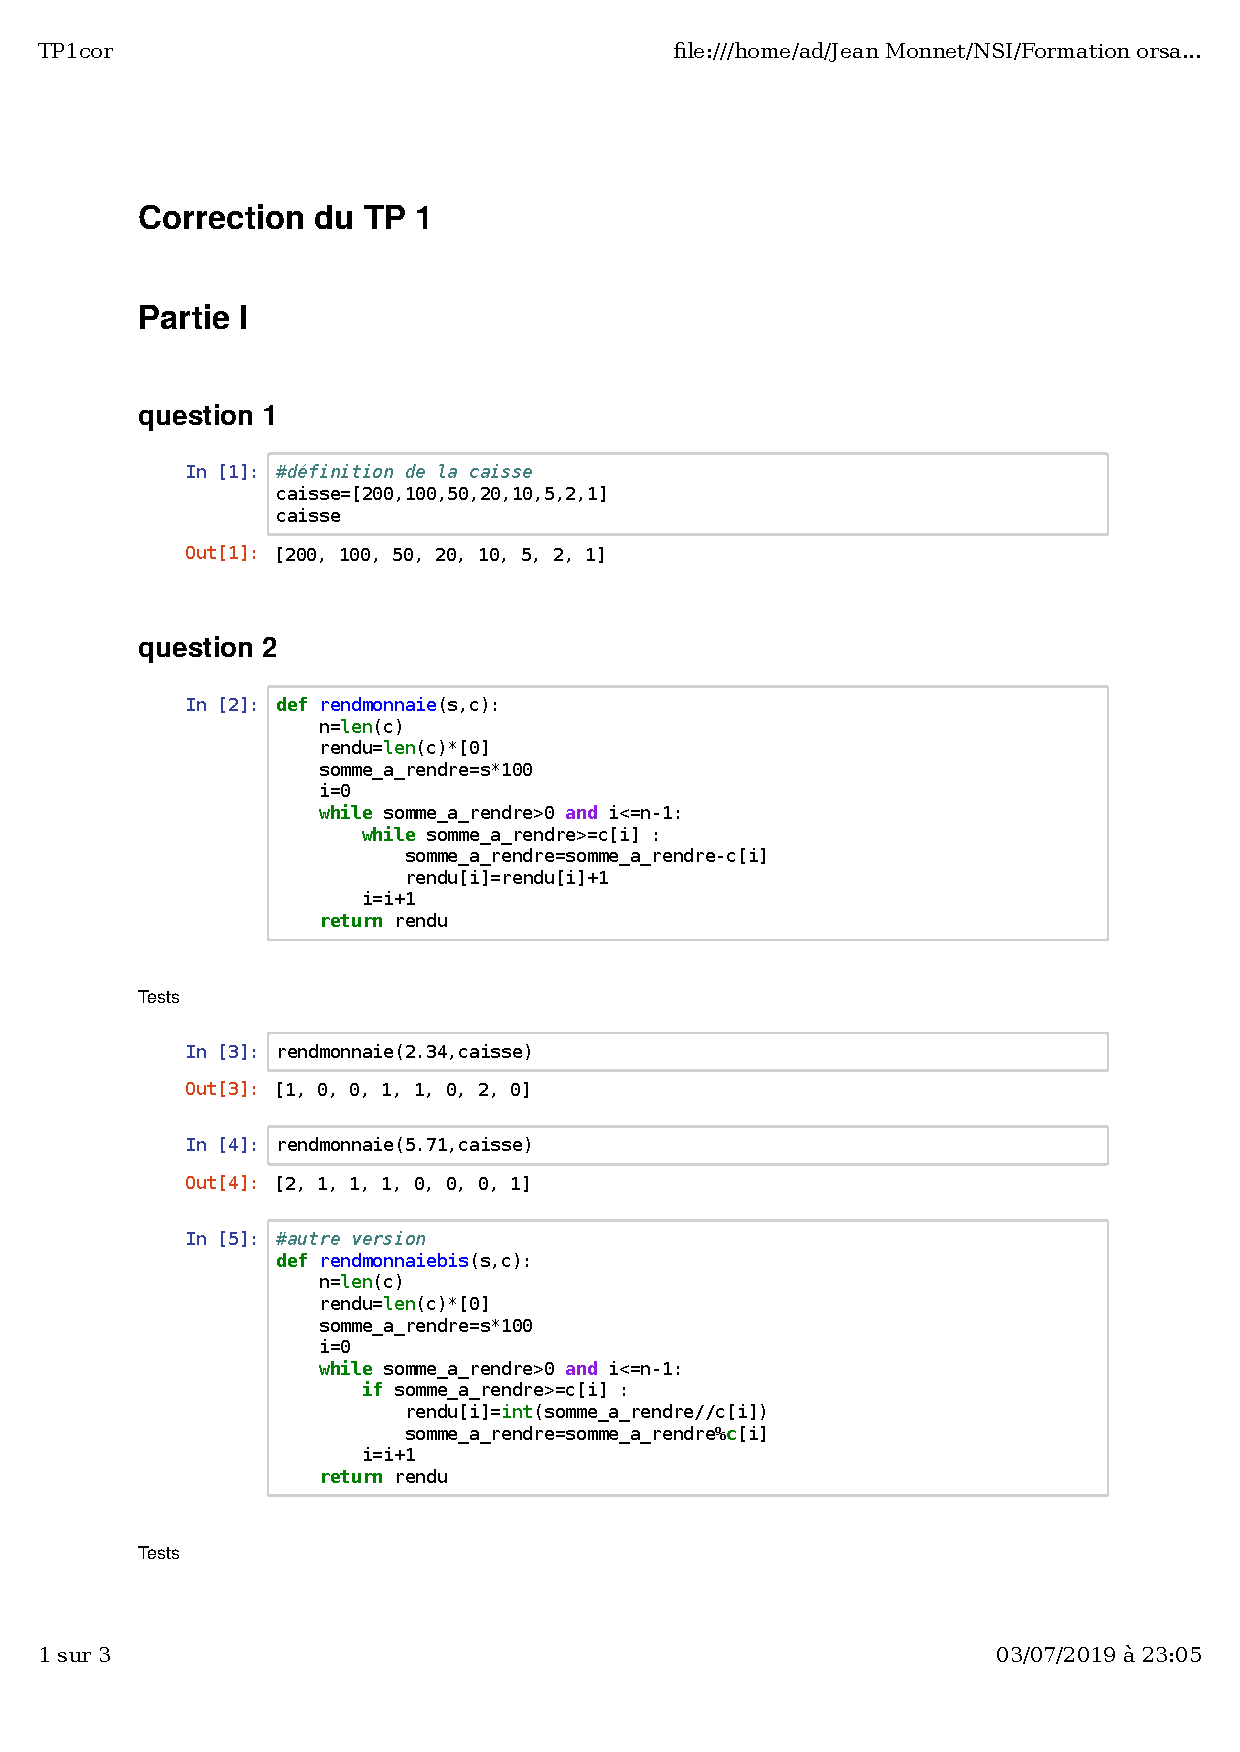
\includepdf[pages=-]{tp1c.pdf}
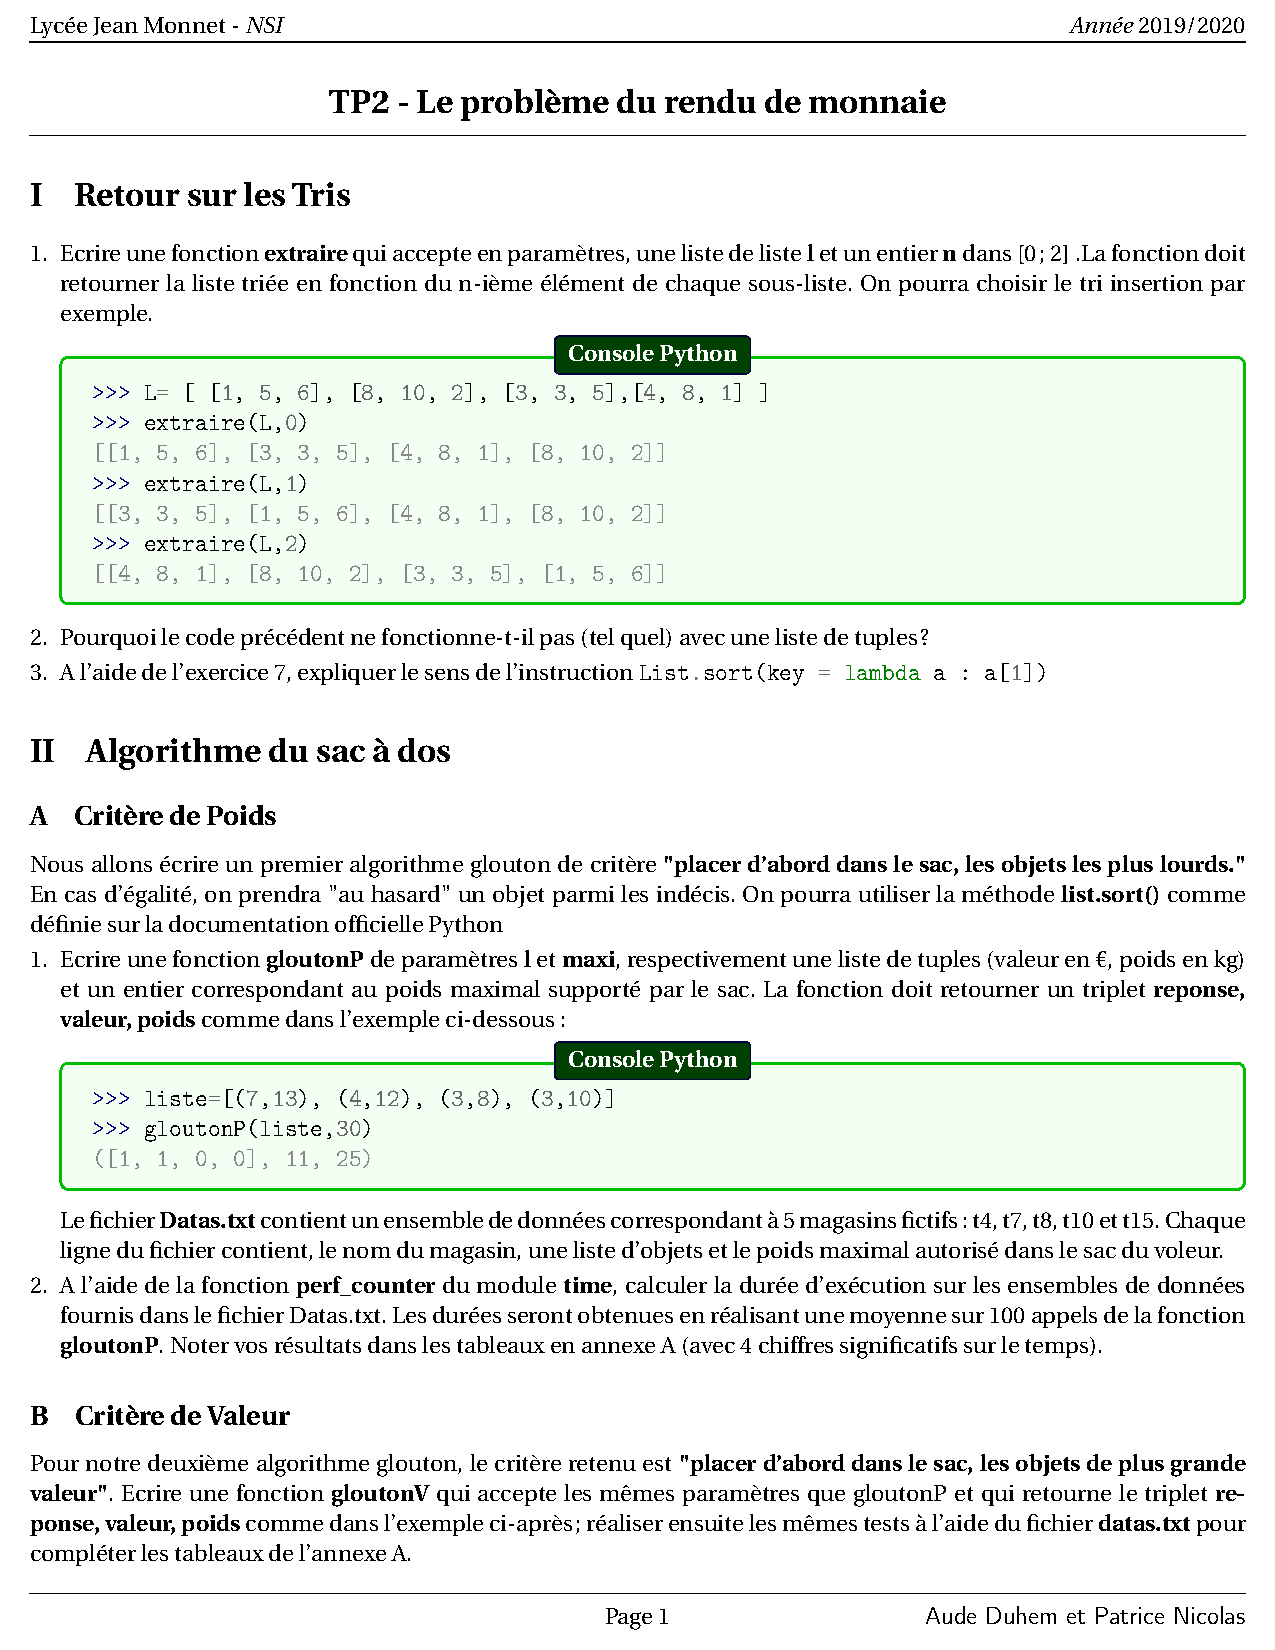
\includepdf[pages=-]{TP2.pdf}
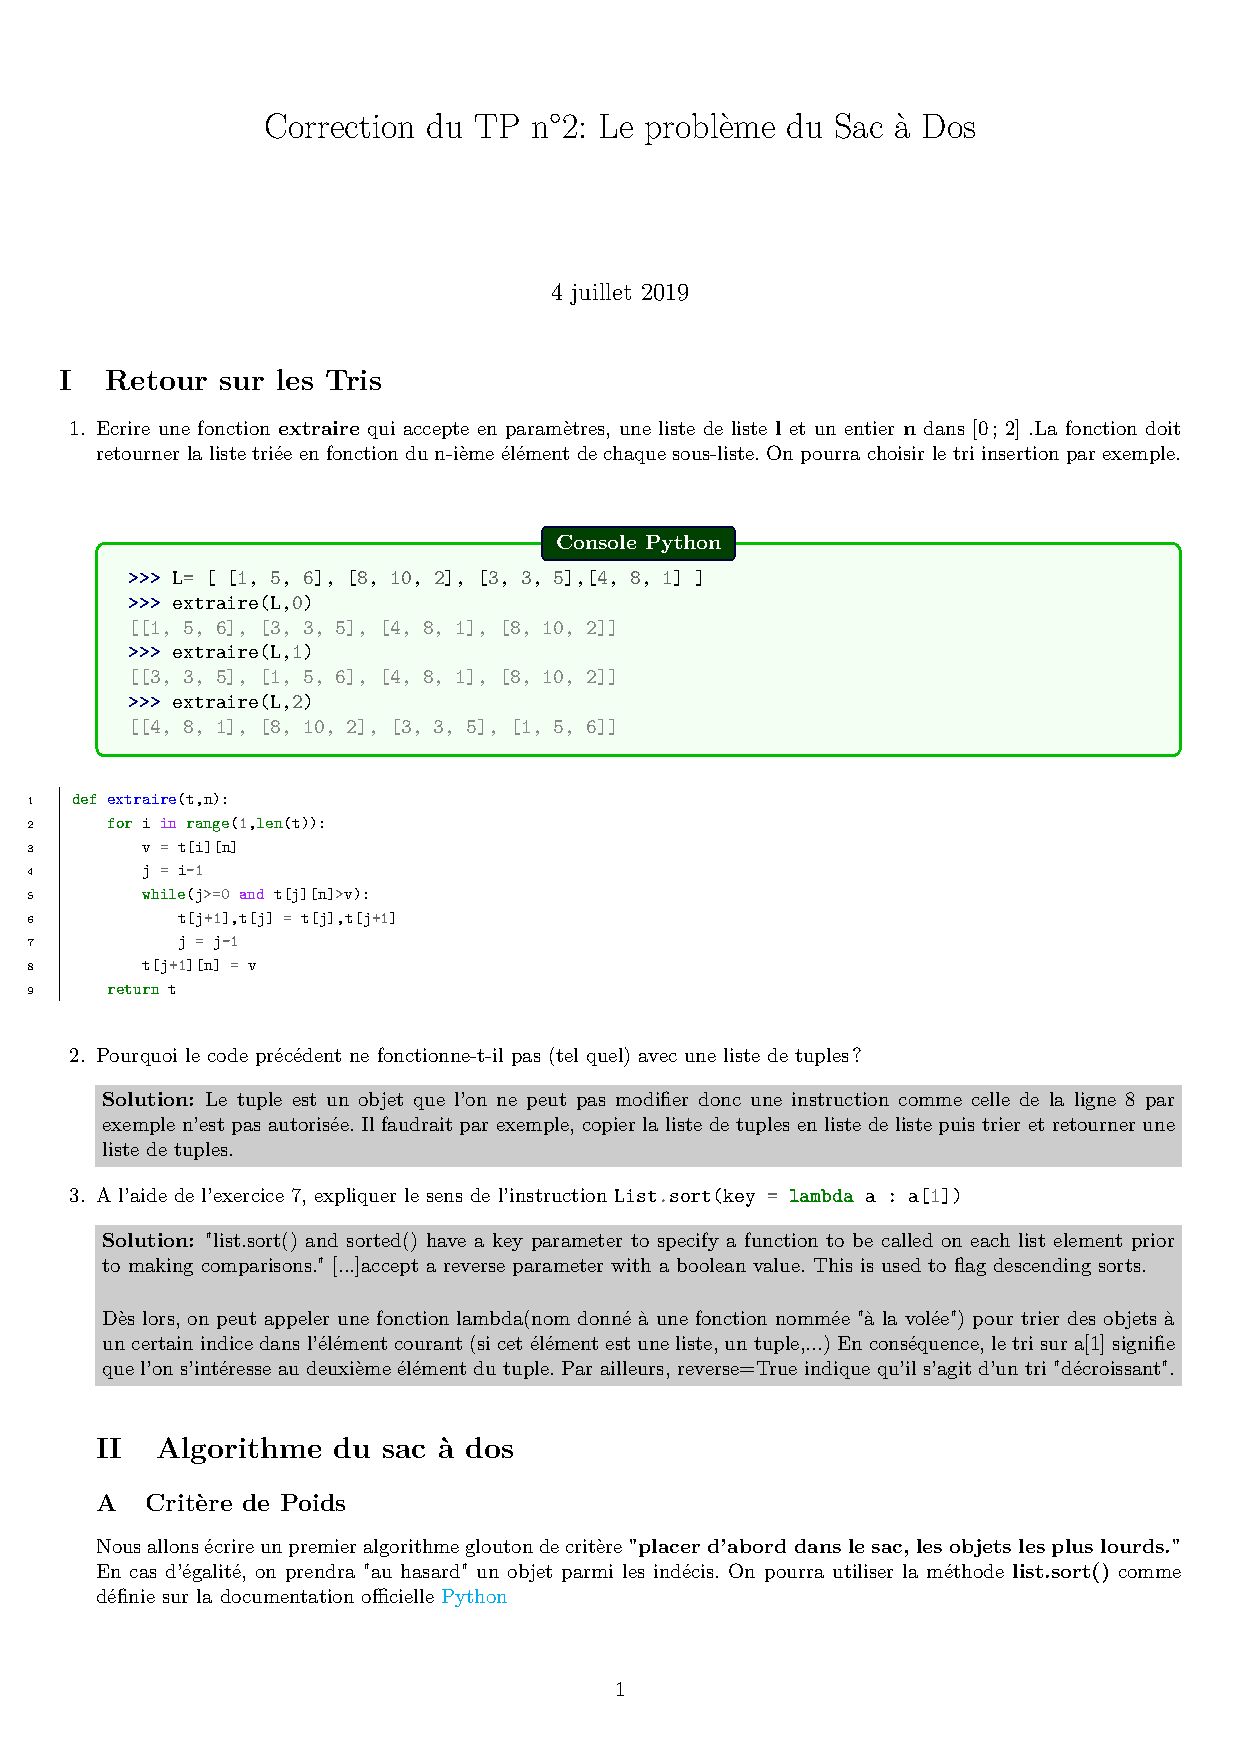
\includepdf[pages=-]{TP2_cor.pdf}
\chapter{Notions mises au lexique}
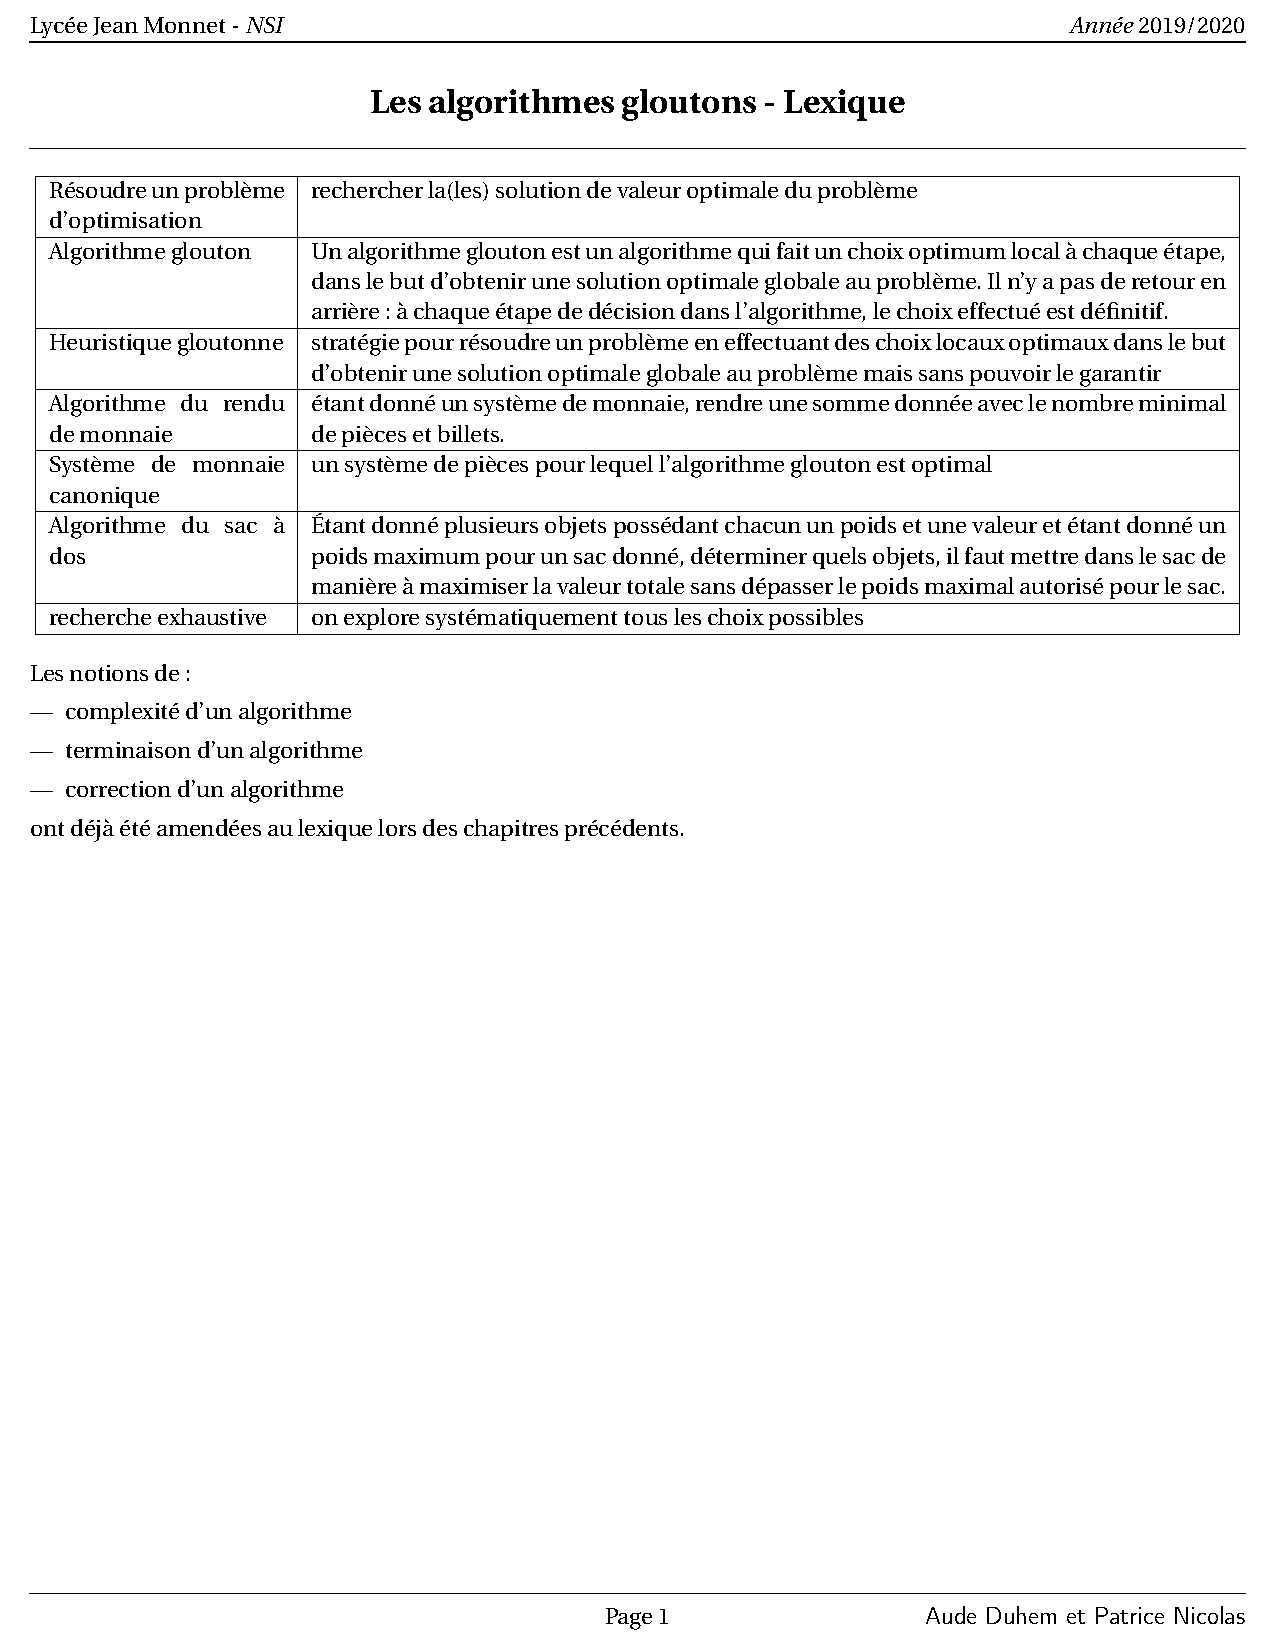
\includepdf[pages=-]{lexique.pdf}
\chapter{Evaluation}
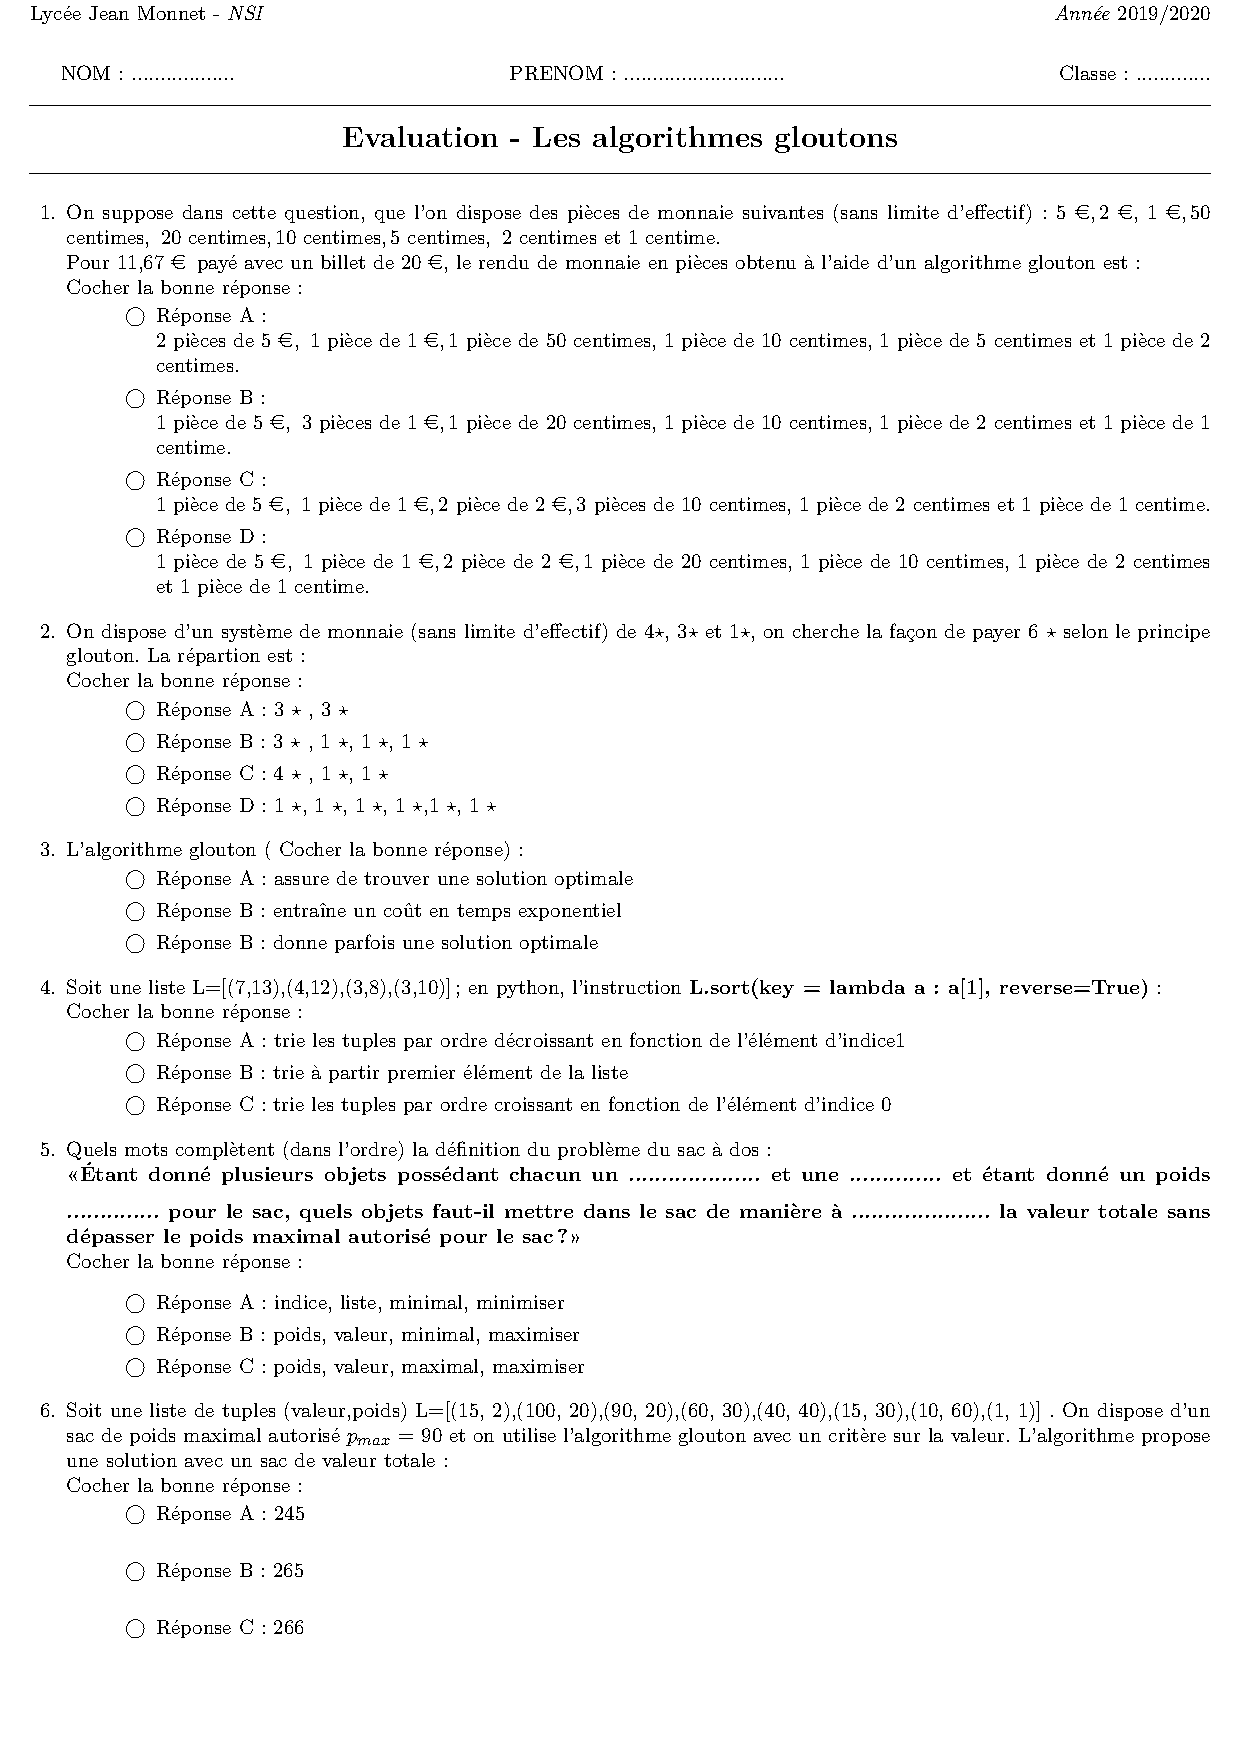
\includepdf[pages=-]{Evaluation.pdf}
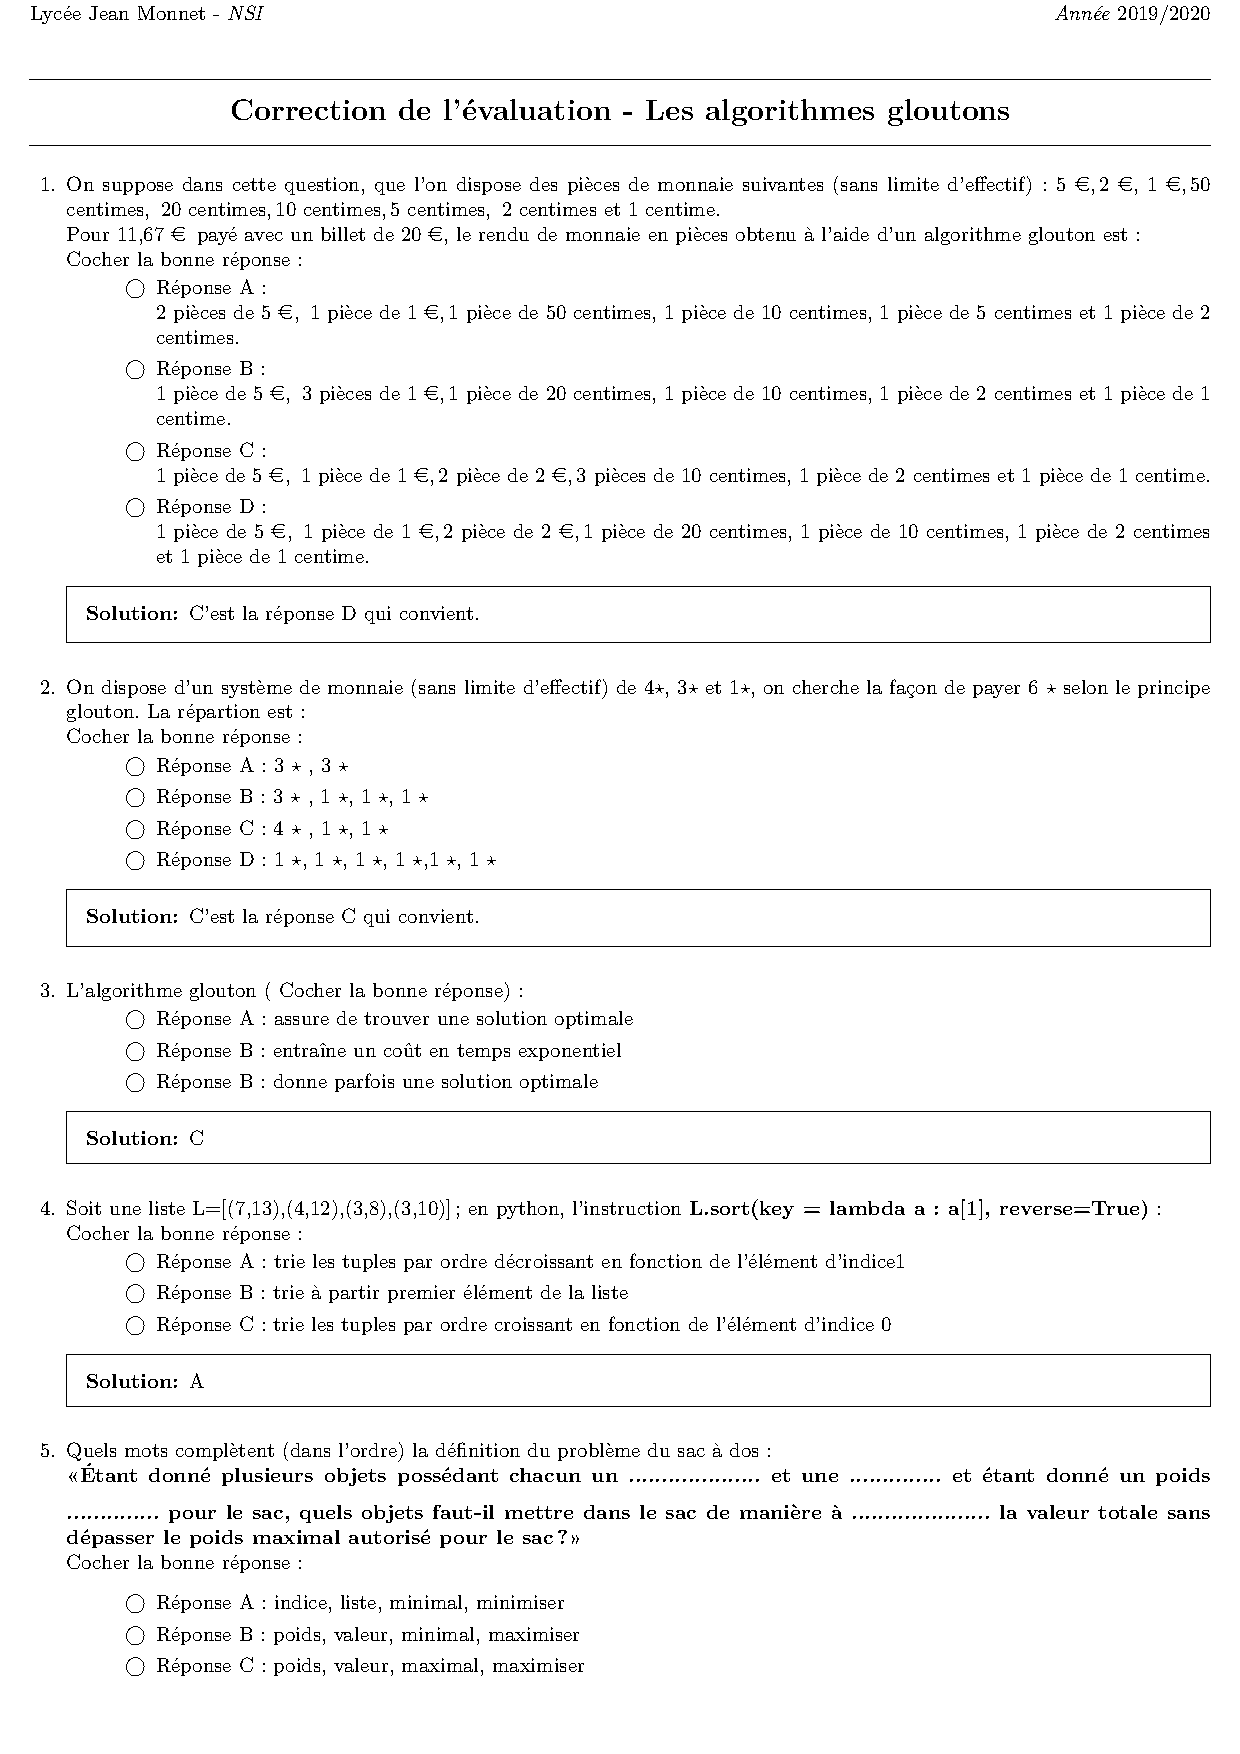
\includepdf[pages=-]{Evaluationcor.pdf}
\chapter{Frise chronologique}
  
\includegraphics{fris}

\end{document}








